\documentclass{beamer}
\usepackage{beamerthemesplit}
\usetheme{SPbGU}
%{CambridgeUS}
% Выпишем часть возможных стилей, некоторые из них могут содержать
% дополнительные опции
% Darmstadt, Ilmenau, CambridgeUS, default, Bergen, Madrid, AnnArbor,Pittsburg, Rochester,
% Antiles, Montpellier, Berkley, Berlin
\usepackage{pdfpages}
\usepackage{amsmath}
\usepackage{cmap} % for serchable pdf's
\usepackage[T2A]{fontenc} 
\usepackage[utf8]{inputenc}
\usepackage[english,russian]{babel}
\usepackage{indentfirst}
\usepackage{amsmath}
\usepackage{dot2texi}
\usepackage{tikz}
\usepackage{fancyvrb}
\usepackage{graphicx}
\usepackage{array}
%\usepackage[usenames,dvipsnames]{color}
\usetikzlibrary{shapes,arrows}
% Если у вас есть логотип вашей кафедры, факультета или университета, то
% его можно включить в презентацию.

%\usefoottemplate{\vbox{}}%  \tinycolouredline{structure!25}% {\color{white}\textbf{\insertshortauthor\hfill% \insertshortinstitute}}% \tinycolouredline{structure}% {\color{white}\textbf{\insertshorttitle}\hfill}% }}

%\logo{\includegraphics[width=1cm]{SPbGU_Logo.png}}

%[GLR-анализатор]
\title[]{Abstract Parsers Generator Based on a Modified RNGLR Algorithm}
%\subtitle[студроект]{Студенческий проект}
\institute[JetBrains]{JetBrains}

\author[Semyon Grigorev]{Semyon Grigorev}

\date{2013г.}

\begin{document}

\begin{frame}
    \begin{tabular}[c с c]{m{2.5cm} m{7cm} m{1.5cm}}
        \begin{center}
        \includegraphics[width=2.5cm]{JBLogoWhite.png}
    \end{center}
    &
    \begin{center}
        \includegraphics[width=7cm]{SLE2013logo.jpg}
    \end{center}
    &
    \begin{center}
        \includegraphics[width=1cm]{SPbGU_Logo.png}
    \end{center}
    \end{tabular}
    \titlepage
\end{frame}

\begin{frame}[fragile]
	\transwipe[direction=90]
	\frametitle{Introduction}
	\begin{itemize}
		\item String-embedded languages:
		\begin{itemize}
		    \item Embedded SQL (in C\#, Java, C++)
		    \item Dynamic SQL
		    \item HTML pages generation
		    \item Other textual DSLs
    	\end{itemize}		
        \item Static analysis of embedded statements.
        \begin{itemize} 
		    \item Syntax errors checking and other analysis:
		    \item IDE support
            \begin{itemize}
    		    \item Syntax highlighting
    		    \item Refactorings
    		    \item Errors notification
        	\end{itemize}
		\end{itemize}
	\end{itemize}
\end{frame}

\definecolor{orange}{RGB}{179,36,31}
\begin{frame}[fragile]
	\transwipe[direction=90]
	\frametitle{String-embedded languages: examples}
	\begin{itemize}
		\item \underline{Dynamic SQL}
		\begin{Verbatim}[commandchars=\\\{\}]
\textcolor{blue}{IF} @X = @Y
    \textcolor{blue}{SET} @TABLE = \textcolor{orange}{'#table1'}
\textcolor{blue}{ELSE}
    \textcolor{blue}{SET} @TABLE = \textcolor{orange}{'table2'}
\textcolor{blue}{EXECUTE} 
    (\textcolor{orange}{'SELECT x FROM'} + @TABLE + \textcolor{orange}{' WHERE ISNULL(n,0) > 1'})
		\end{Verbatim}
		\item \underline{JavaScript in Java}
		\begin{Verbatim}[commandchars=\\\{\}]
\textcolor{blue}{String} script =
    \textcolor{orange}{"function hello(name) { print(’Hello, ’ + name); }"};
engine.eval(script);
\textcolor{blue}{Invocable} inv = (\textcolor{blue}{Invocable}) engine;
inv.invokeFunction(\textcolor{orange}{"hello"}, \textcolor{orange}{"Scripting!!!"} );
        \end{Verbatim}
	\end{itemize}
\end{frame}

\begin{frame}[fragile]
	\transwipe[direction=90]
	\frametitle{Abstract parsing}
	Main points of “classical” abstract parsing
	\begin{itemize}
	    \item Based on (G)LR algorithm
	    \begin{itemize}
            \item Tables generator could be reused.
        \end{itemize}
        \item Additional data structures
        \begin{itemize}
            \item “Abstract” stack
            \item Parsing forest
        \end{itemize}
    \end{itemize}
    There is a set of tools based on it.
    \begin{itemize}
        \item Alvor: Eclipse plug-in for SQL ebedded into Java checking.
        \item Java String Analyzer: tool for analyzing the flow of strings and string operations in Java programs.
        \item PHP String Analyzer: static program analyzer that approximates the string output of a PHP program.
    \end{itemize}
\end{frame}

\begin{frame}[fragile]
	\transwipe[direction=90]
	\frametitle{GLR parsing}
	\begin{itemize}
	    \item For ambiguous CFG processing. 
	    \item Shift$\backslash$Reduce and Reduce$\backslash$Reduce conflicts.
	    \item Graph Structured Stack -- GSS.
    	\begin{itemize}
	        \item Branches on conflicts.
	        \item States merging.
        \end{itemize}
    \end{itemize}
\end{frame}

\begin{frame}[fragile]
	\transwipe[direction=90]
	\frametitle{Our approach}
	\begin{itemize}
	    \item We work with RNGLR -- Right Nulled GLR.
        \item Shift$\backslash$Shift conflicts — branches in input “stream”. Impossible for sequential input.
        \begin{itemize}
    	    \item RNGLR should be extended for process this conflicts.
	    \end{itemize}
        \item Reusing of inner structures: GSS and parsing result (graph-structured also).
        \begin{itemize}
            \item Shift$\backslash$Shift conflicts — new branches in GSS.
            \item Parsing result is a graph which contains all possible trees.
        \end{itemize}
    \end{itemize}
\end{frame}

\begin{frame}[fragile]
	\transwipe[direction=90]
	\frametitle{Example: input}
	\begin{itemize}
	    \item Grammar:
    	\begin{verbatim}
s: NUM PLUS e
e: NUM
        \end{verbatim}
	    \item Input graph:
	    \begin{center}
            \begin{dot2tex}[dot]
                digraph G
                {
                    d2toptions="--autosize";
                    rankdir=LR
                    0 -> 1 [label = "NUM(1)"]
                    0 -> 2 [label = "NUM(2)"]
                    1 -> 3 [label = "PLUS"]
                    2 -> 3 [label = "PLUS"]
                    3 -> 4 [label = "NUM(3)"]
                 }
             \end{dot2tex}
	    \end{center}
    \end{itemize}
\end{frame}

\begin{frame}[fragile]
	\transwipe[direction=90]
	\frametitle{Example: stack}
%	    \begin{center}
            \begin{dot2tex}[dot]
            digraph GSS2 {
                d2toptions="--autosize";
                rankdir=RL
                0 [label="\ ",texlbl=" \ ", color=white]
                1 [label="0"]
                0 -> 1 [label="3",texlbl="\ ", color=white]
                2 [label=" \ ",texlbl="\ ",color=white]
                3 [label=" ",texlbl="\ ",color=white]
                4 [label="2",texlbl="\ ",color=white]
                4 -> 1 [label="NUM(1)",texlbl="\ \ \ \ \ ",color=white]
                3 -> 4 [label="PLUS",texlbl="\ \ \ \ \ ",color=white]
                5 [label=" ",texlbl="\ ",color=white]
                5 -> 1 [label="NUM(1)",texlbl="\ \ \ \ \ ",color=white]
                3 -> 5 [label="PLUS",texlbl="\ \ \ \ \ ",color=white]
                2 -> 3 [label="3",texlbl="\ ",color=white]
                6 [texlbl="\ ",color=white]
                6 -> 3 [label="NUM(4)",texlbl="\ \ \ \ \ ",color=white]
                {rank=same; 6 2 0}
                {rank=same; 1}
                {rank=same; 3}
                {rank=same; 4}
                {rank=same; 5}
            }
            \end{dot2tex}
%	    \end{center}
\end{frame}


\begin{frame}[fragile]
	\transwipe[direction=90]
	\frametitle{Example: stack}
%	    \begin{center}
            \begin{dot2tex}[dot]
            digraph GSS2 {
                d2toptions="--autosize";
                rankdir=RL
                0 [label="\ ",texlbl=" \ ", color=white]
                1 [label="0"]
                0 -> 1 [label="3",texlbl="\ ", color=white]
                2 [label=" \ ",texlbl="\ ",color=white]
                3 [label=" ",texlbl="\ ",color=white]
                4 [label="2"]
                4 -> 1 [label="NUM(1)"]
                3 -> 4 [label="PLUS",texlbl="\ \ \ \ \ ",color=white]
                5 [label=" ",texlbl="\ ",color=white]
                5 -> 1 [label="NUM(1)",texlbl="\ \ \ \ \ ",color=white]
                3 -> 5 [label="PLUS",texlbl="\ \ \ \ \ ",color=white]
                2 -> 3 [label="3",texlbl="\ ",color=white]
                6 [texlbl="\ ",color=white]
                6 -> 3 [label="NUM(4)",texlbl="\ \ \ \ \ ",color=white]
                {rank=same; 6 2 0}
                {rank=same; 1}
                {rank=same; 3}
                {rank=same; 4}
                {rank=same; 5}
            }
            \end{dot2tex}
%	    \end{center}
\end{frame}


\begin{frame}[fragile]
	\transwipe[direction=90]
	\frametitle{Example: stack}
%	    \begin{center}
            \begin{dot2tex}[dot]
            digraph GSS2 {
                d2toptions="--autosize";
                rankdir=RL
                0 [label="\ ",texlbl=" \ ", color=white]
                1 [label="0"]
                0 -> 1 [label="3",texlbl="\ ", color=white]
                2 [label=" \ ",texlbl="\ ",color=white]
                3 [label="3"]
                4 [label="2"]
                4 -> 1 [label="NUM(1)"]
                3 -> 4 [label="PLUS"]
                5 [label=" ",texlbl="\ ",color=white]
                5 -> 1 [label="NUM(1)",texlbl="\ \ \ \ \ ",color=white]
                3 -> 5 [label="PLUS",texlbl="\ \ \ \ \ ",color=white]
                2 -> 3 [label="3",texlbl="\ ",color=white]
                6 [texlbl="\ ",color=white]
                6 -> 3 [label="NUM(4)",texlbl="\ \ \ \ \ ",color=white]
                {rank=same; 6 2 0}
                {rank=same; 1}
                {rank=same; 3}
                {rank=same; 4}
                {rank=same; 5}
            }
            \end{dot2tex}
%	    \end{center}
\end{frame}

\begin{frame}[fragile]
	\transwipe[direction=90]
	\frametitle{Example: stack}
%	    \begin{center}
            \begin{dot2tex}[dot]
            digraph GSS2 {
                d2toptions="--autosize";
                rankdir=RL
                0 [label=" ", color=white]
                1 [label="0"]
                0 -> 1 [label=" ", color=white]
                2 [label=" ",color=white]
                3 [label="3"]
                4 [label="2"]
                4 -> 1 [label="NUM(1)"]
                3 -> 4 [label="PLUS"]
                5 [label="2"]
                5 -> 1 [label="NUM(2)"]
                3 -> 5 [label="    ",color=white]
                2 -> 3 [label=" ",color=white]
                6 [label=" ",color=white]
                6 -> 3 [label="       ",color=white]
                {rank=same; 6 2 0}
                {rank=same; 1}
                {rank=same; 3}
                {rank=same; 4}
                {rank=same; 5}
            }
            \end{dot2tex}
%	    \end{center}
\end{frame}

\begin{frame}[fragile]
	\transwipe[direction=90]
	\frametitle{Example: stack}
%	    \begin{center}
            \begin{dot2tex}[dot]
            digraph GSS2 {
                d2toptions="--autosize";
                rankdir=RL
                0 [label=" ", color=white]
                1 [label="0"]
                0 -> 1 [label=" ", color=white]
                2 [label=" ",color=white]
                3 [label="3"]
                4 [label="2"]
                4 -> 1 [label="NUM(1)"]
                3 -> 4 [label="PLUS"]
                5 [label="2"]
                5 -> 1 [label="NUM(2)"]
                3 -> 5 [label="PLUS"]
                2 -> 3 [label=" ",color=white]
                6 [label=" ",color=white]
                6 -> 3 [label="       ",color=white]
                {rank=same; 6 2 0}
                {rank=same; 1}
                {rank=same; 3}
                {rank=same; 4}
                {rank=same; 5}
            }
            \end{dot2tex}
%	    \end{center}
\end{frame}

\begin{frame}[fragile]
	\transwipe[direction=90]
	\frametitle{Example: stack}
%	    \begin{center}
            \begin{dot2tex}[dot]
            digraph GSS2 {
                d2toptions="--autosize";
                rankdir=RL
                0 [label=" ", color=white]
                1 [label="0"]
                0 -> 1 [label=" ", color=white]
                2 [label=" ",color=white]
                3 [label="3"]
                4 [label="2"]
                4 -> 1 [label="NUM(1)"]
                3 -> 4 [label="PLUS"]
                5 [label="2"]
                5 -> 1 [label="NUM(2)"]
                3 -> 5 [label="PLUS"]
                2 -> 3 [label=" ",color=white]
                6 [label="5"]
                6 -> 3 [label="NUM(3)"]
                {rank=same; 6 2 0}
                {rank=same; 1}
                {rank=same; 3}
                {rank=same; 4}
                {rank=same; 5}
            }
            \end{dot2tex}
%	    \end{center}
\end{frame}

\begin{frame}[fragile]
	\transwipe[direction=90]
	\frametitle{Example: stack}
%	    \begin{center}
            \begin{dot2tex}[dot]
            digraph GSS2 {
                d2toptions="--autosize";
                rankdir=RL
                0 [label=" ", color=white]
                1 [label="0"]
                0 -> 1 [label=" ", color=white]
                2 [label="4"]
                3 [label="3"]
                4 [label="2"]
                4 -> 1 [label="NUM(1)"]
                3 -> 4 [label="PLUS"]
                5 [label="2"]
                5 -> 1 [label="NUM(2)"]
                3 -> 5 [label="PLUS"]
                2 -> 3 [label="e"]
                6 [label="5"]
                6 -> 3 [label="NUM(3)"]
                {rank=same; 6 2 0}
                {rank=same; 1}
                {rank=same; 3}
                {rank=same; 4}
                {rank=same; 5}
            }
            \end{dot2tex}
%	    \end{center}
\end{frame}

\begin{frame}[fragile]
	\transwipe[direction=90]
	\frametitle{Example: stack}
%	    \begin{center}
            \begin{dot2tex}[dot]
            digraph GSS {
                d2toptions="--autosize";
                rankdir=RL
                0 [label="1"]
                1 [label="0"]
                0 -> 1 [label="s"]
                2 [label="4"]
                3 [label="3"]
                4 [label="2"]
                4 -> 1 [label="NUM(1)"]
                3 -> 4 [label="PLUS"]
                5 [label="2"]
                5 -> 1 [label="NUM(2)"]
                3 -> 5 [label="PLUS"]
                2 -> 3 [label="e"]
                6 [label="5"]
                6 -> 3 [label="NUM(3)"]
                {rank=same; 6 2 0}
                {rank=same; 1}
                {rank=same; 3}
                {rank=same; 4}
                {rank=same; 5}
            }
            \end{dot2tex}
%	    \end{center}
\end{frame}

\begin{frame}[fragile]
	\transwipe[direction=90]
	\frametitle{Example: parsing result}
    \begin{center}
            \begin{dot2tex}[dot]
            digraph AST {
                d2toptions="--autosize";
                1 [label="s",style="filled",fillcolor=red,shape=box]
                5 [label="prod 0"]
                1 -> 5 [style=bold,width=10,label=""]
                6 [label="t NUM",shape=box]
                5 -> 6 [label=""]
                7 [label="t PLUS",shape=box]
                5 -> 7 [label=""]
                5 -> 0 [label=""]
                8 [label="prod 0"]
                1 -> 8 [style=bold,width=10,label=""]
                9 [label="t NUM",shape=box]
                8 -> 9 [label=""]
                10 [label="t PLUS",shape=box]
                8 -> 10 [label=""]
                8 -> 0 [label=""]
                0 [label="e",shape=box]
                12 [label="t NUM",shape=box]
                0 -> 12 [label=""]
            }
        \end{dot2tex}
    \end{center}
\end{frame}

\begin{frame}[fragile]
	\transwipe[direction=90]
	\frametitle{Results}
	\begin{itemize}
	    \item Abstract parsing algorithm based on modified RNGLR is implemented.
	    \begin{itemize}
	        \item GSS is reused.
	        \item Compact inner representation of parsing results with node reusing is used.
            \item Parsers geneartor is implemented.
        \end{itemize}
	    \item Plug-in for ReSharper in active development.
	    \begin{itemize}
	        \item  Modular architecture is allow to create extensions for any string-embedded language.
        \end{itemize}
	\end{itemize}
\end{frame}

\begin{frame}[fragile]
	\transwipe[direction=90]
	\frametitle{Demo}
	\begin{center}
	    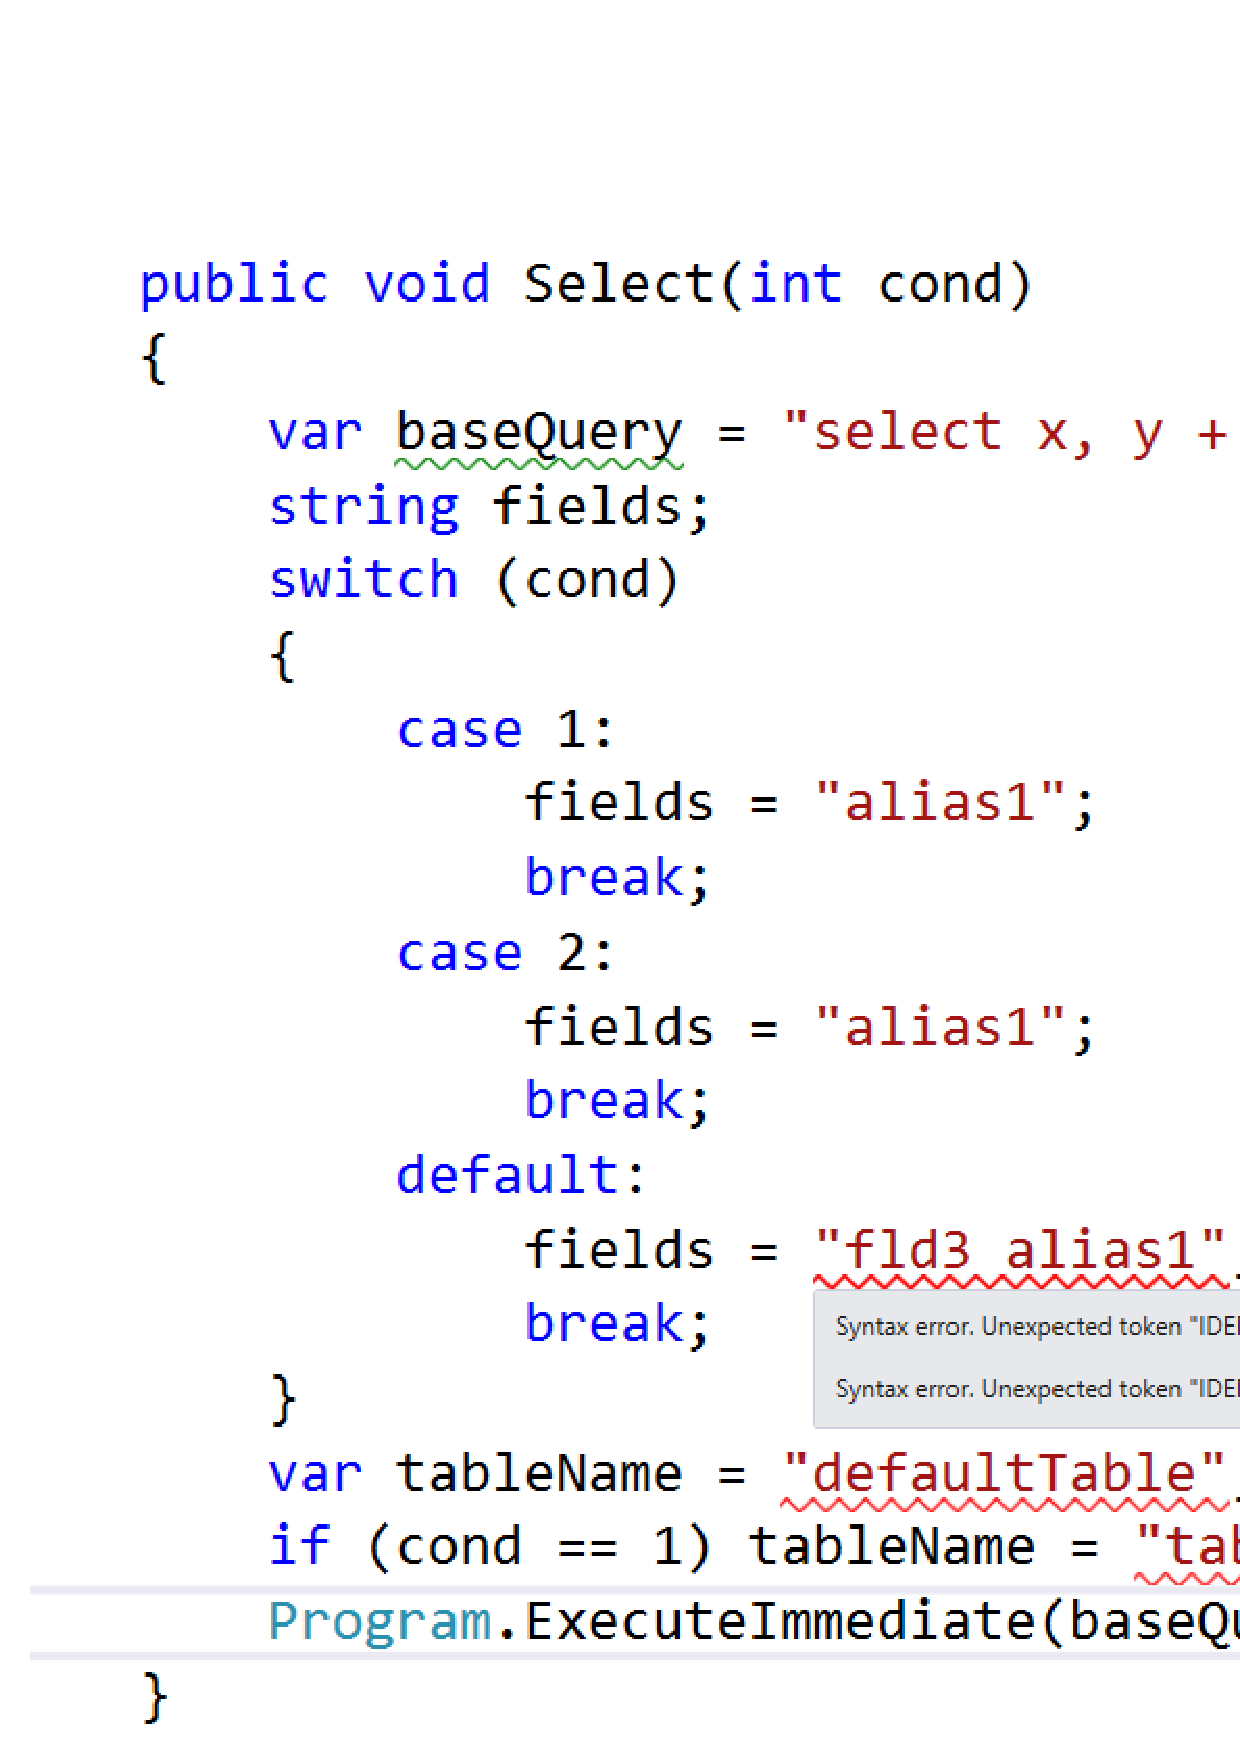
\includegraphics[width=290pt]{Screen1.png}
	\end{center}
\end{frame}

\begin{frame}
	\transwipe[direction=90]
	\frametitle{Contacts}
	\begin{itemize}
		\item Semyon Grigorev:
		\begin{itemize}
    		\item Semen.Grigorev@jetbrains.com
    		\item rsdpisuy@gmail.com
    	\end{itemize}		
		\item YaccConstructor: \href{http://recursive-ascent.googlecode.com}{http://recursive-ascent.googlecode.com}
	\end{itemize}
\end{frame}

\end{document}
